\documentclass[journel,12pt,twocoloums]{IEEEtran}

\title{Assignment 8-Probability and Random Variable}
\author{Annu-EE21RESCH01010}
\date{13 January 2020}

\usepackage{amsthm}
\usepackage{graphicx}
\usepackage{mathrsfs}
\usepackage{txfonts}
\usepackage{stfloats}
\usepackage{pgfplots}
\usepackage{cite}
\usepackage{cases}
\usepackage{mathtools}
\usepackage{caption}
\usepackage{enumerate}	
\usepackage{enumitem}
\usepackage{amsmath}
\usepackage[utf8]{inputenc}
\usepackage[english]{babel}
\usepackage{multicol}
%\usepackage{xtab}
\usepackage{longtable}
\usepackage{multirow}
%\usepackage{algorithm}
%\usepackage{algpseudocode}
\usepackage{array,multirow}
\usepackage{enumitem}
\usepackage{mathtools}
\usepackage{gensymb}
\usepackage{hyperref}
%\usepackage[framemethod=tikz]{mdframed}
\usepackage{listings}
    %\usepackage[latin1]{inputenc}                                 %%
    \usepackage{color}                                            %%
    \usepackage{array}                                            %%
    \usepackage{longtable}                                        %%
    \usepackage{calc}                                             %%
    \usepackage{multirow}                                         %%
    \usepackage{hhline}                                           %%
    \usepackage{ifthen}                                         %%
  \providecommand{\nCr}[2]{\,^{#1}C_{#2}}
  \providecommand{\nPr}[2]{\,^{#1}P_{#2}}
  \lstset{
%language=C,
frame=single, 
breaklines=true,
columns=fullflexible
}

 \begin{document}
 \maketitle
\textbf{Download latex code from here-}\\
\begin{lstlisting}
 https://github.com/annu100/AI5002-Probability-and-Random-variables/tree/main/ASSIGNMENT_8
 \end{lstlisting}
 \textbf{Download python code from here-}\\
\begin{lstlisting}
 https://github.com/annu100/AI5002-Probability-and-Random-variables/tree/main/ASSIGNMENT_8
 \end{lstlisting}
 \section{Problem Statement-Problem 6.18}

If  P(A) =$\frac{7}{13}$,
, P(B) =$\frac{9}{13}$
and 
P(A $\cap$ B) = $\frac{4}{13}$.
Evaluate P(A/B)?
Simulation part -
Also generate random variables according to 2 given probabilities and using simulated probabilities ,calculate P(A/B) and cross check with actual result of P(A/B) using baye's theoram formula.
\section{SOLUTIONS}
\subsection{Probability calculation}
We know that for independent random variables,multiplication of probability 2 random variables must be equal to multiplication of individual probability of those random variables.
P(A) =$\frac{7}{13}$
P(B) =$\frac{9}{13}$
P(A $\cap$ B) =$\frac{4}{13}$
From baye's theoram ,we know that P(A/B)=P(A $\cap$ B)/P(B)
\begin{align}
         P(A/B) &= P(A \cap B)/P(B) \\
                &=(\frac{4}{13})/(\frac{9}{13})\\
                &=\frac{4}{9}
\end{align}
\\
Therefore,P(A/B)=$\frac{4}{9}$
\begin{figure}

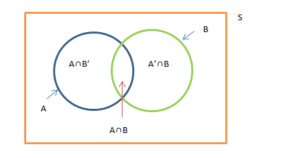
\includegraphics[width=\columnwidth] {independence.png}


\end{figure}


\subsection{Simulation using Random variables geeneration}
\\
\\
\\


Now generating numtrials=100 samples according to 2 given probability distribution described in above table.\\
Generated samples according to the probability distribution is 

['1', '0', '1', '0', '1', '1', '1', '0', '0', '0', '1', '0', '0', '1', '1', '1', '0', '0', '0', '0', '1', '1', '1', '0', '0', '0', '0', '1', '0', '1', '1', '1', '1', '1', '0', '1', '1', '0', '1', '1', '1', '1', '1', '1', '0', '1', '1', '1', '0', '0', '1', '1', '0', '1', '1', '0', '0', '0', '1', '1', '1', '0', '0', '1', '1', '1', '0', '0', '0', '1', '1', '0', '0', '0', '1', '0', '0', '0', '1', '1', '1', '0', '0', '1', '1', '0', '0', '0', '1', '1', '1', '0', '1', '1', '0', '0', '0', '0', '0', '0']\\
\subsection{Simulation using Random variables generation Results}
simulation versus actual probabilities\\
Actual probabilities i.e P(A),P(B)are [0.5384615384615384, 0.6923076923076923]\\
simulation probabilities are given by \\

Probability for X=0 i.e P(A)is  0.48\\
Probability for X=1 i.e P(B)is  0.52\\
simulation versus actual probabilities for P(A/B)\\
simulated prob is i.e P(A/B) 0.591715976331361\\
using baye''s probabilities i.e P(A/B)is 
 0.4444444444444445\\
 
 \begin{figure}

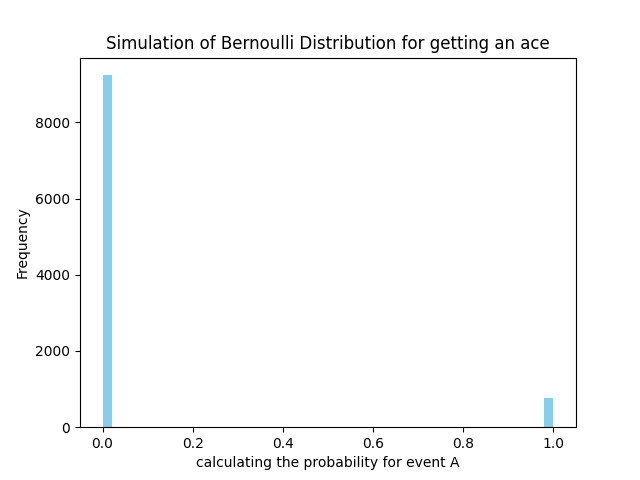
\includegraphics[width=\columnwidth] {Figure_1.png}


\end{figure}
We can increase the number of samples in order to get more appropriate results.Here, graph is linear which is implying same i. e simulated and actual probability  More linear implies more appropriate result.
\end{document}

        

